\chapter{Implementation}\label{C:imp}
The implementation process took the planned designs and selected hardware and constructing an integrated system. This provided an opportunity to test, iterate finalise the designs and approaches of the project.      

\section{Mechanical Components}
Implementing the mechanical components of the system covered the material choice, manufacture and adjustment of the motor mounting brackets, shaft couplers and interfacing and pipette mounting and supports. Considerations taken were speed of iterations. Flexibility in adapting specific dimensions to suit needs and to maximise reliability and stability. 

\subsection{Rotating Pipette Mount}
The C-clamp's design did not fundamentally change from the initial design, and remained the duel clamping system with matched internal circumferences. They did however go through many smaller interactions to achieve the preferred performance. Firstly, obtaining the required internal circumference of the clamps from the asymmetric body of the pipette was taken using a length of string was used to at the points of intended fastening. The clamping pressure then deformed the initially circular parts to the ergonomic form of the pipette body.

\begin{wrapfigure}{r}{0.3\textwidth}
    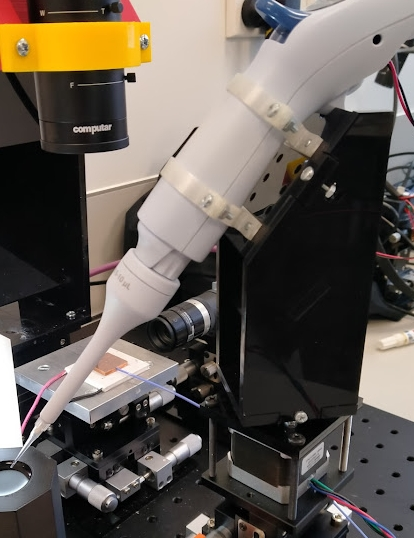
\includegraphics[width=0.25\textwidth]{img/r_pip.jpg}
    \caption{Final constructed Pipette stage mounting tower w/ clamps and motor}
\end{wrapfigure}

This process, and the resulting measurements of 32mm and 36mm remained unchanged.
However, the ring thickness was varied and tested. 3 options were 3D printed and trialled; 1mm, 1.5mm, and 2mm. This thickness affected the clamps ability to deform to the shape of the pipette, how rigid the mounting was and the strength at the clamping screw holes.

1mm was used for the longest initially, but had a noticeable woggle as well and resulting in the screw hole delaminating from the ring due to flexing in the plastic. After this failure, the 1.5 and 2mm versions were printed and trialled for a shorter period. The 2mm provided much better strength, showing no noticeable degradation at points of high-stress concentration. However where this thickness failed was in deforming, the added rigidity was just too inflexible to ever fully clamp and resulted in play/slippage. Given this, two 1.5mm version were printed to compromise and successfully deformed and remained intact over the remaining project time.   

Another area of tweaking was the screw tolerance. These pieces were designed to take advantage of the plastics deformation to also allow for the screws to cut their own threads as provide a stronger grip. As the screw is initially inserted a too smaller hole can result in splitting delamination of the plastic layers, via experimentation, a +0.2mm diameter tolerance allowed for retaining that 'self-tapping' characteristic while maintaining structural integrity. 

The tower itself was designed to be fully laser cut from acrylic to minimise [material] flexibility and to aid to modularity. This allowed the height to be adjustable by cutting different side pieces for example. This did not deviate from design, but initially, the tower was glued together to reduce weight but this was quickly scrapped for machine screw bolting, with the intention that any oscillations or resonance in the system would be tuned for on the motor driving side of the project.

\subsection{Z micrometer Control}

The Z height adjustment represents the most sensitive mechanical system and required careful measurements to axially align the micrometer knob and the shaft as well as matching the coupler length to accommodate the discrete fastening points of the optical breadboard. 

\begin{wrapfigure}{r}{0.42\textwidth}
    \centering
    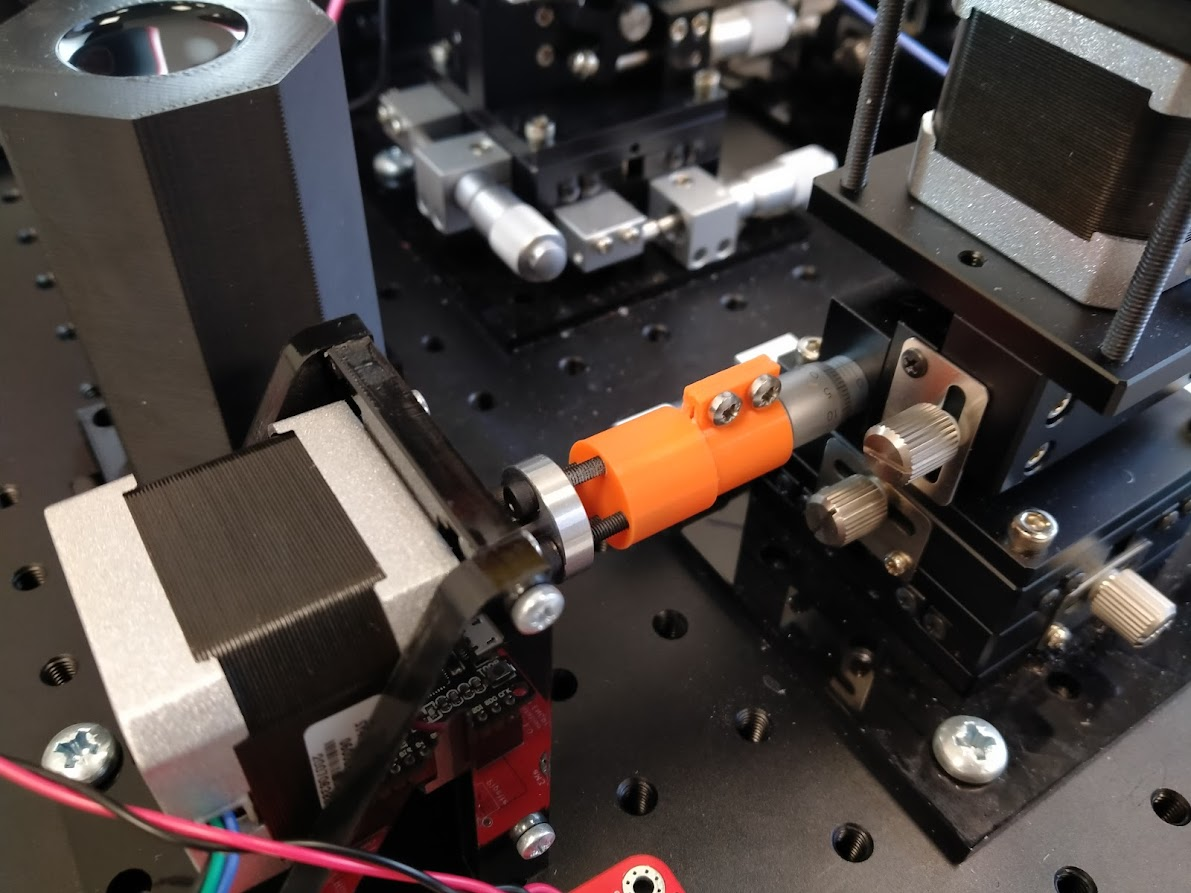
\includegraphics[width=0.4\textwidth]{img/impl_coup.jpg}
    \caption{Constructed Motor mount and sliding coupler interfacing with the z-micrometer of the XYZ stage}
    \label{fig:z_coup}
\end{wrapfigure}

The figure above \ref{fig:z_coup}shows the Z-motor statically mounted to the breadboard with a laser-cut bracket assembly. This, along with the aforementioned tight tolerance requires presented the first problem to overcome with mechanical performance.

The initial z-coupler was printed with a 1mm defect in it radius as too small M3 screw holes. This cause splitting under high load as well as large vibrations that propagated through the whole system as was causing premature droplet detachment.

After reprinting the coupler, these vibrations were greatly reduced by still present. To combat this, the motor driving parameters were adjusted, slowing the signal speed from 10 revolutions per second until it no longer resonated during the adjustment. Final parameters were 6 rev/s and 100 rev/s/s.

\section{Electronic Components}

The aim of the electronics in this project is to provide an interface for the host computer to send commands with the controlling microcontroller and supply and support the stepper driving stages and their required current. The microcontroller receives command strings over serial USB and parsed them and executes them either at PWM control signals to the STEP inputs of the drivers or digital flag signals to the pipette. The driver requires a motor supply voltage of 8.2 – 45 V. This supply should have appropriate decoupling capacitors close to the board, and it should be capable of delivering the expected stepper motor current.

These decoupling capacitors are to act as reservoirs for high loads and shield the onboard low-ESR ceramics from LC voltage spikes. These spikes can exceed the 45 V maximum voltage rating for the DRV8825 and permanently damage the board, even when the motor supply voltage is as low as 12 V. This was addressed with the addition of  a pair of 100u electrolytic capacitors across the motor power rails right next to the carriers.

\begin{figure}[h]
    \centering
    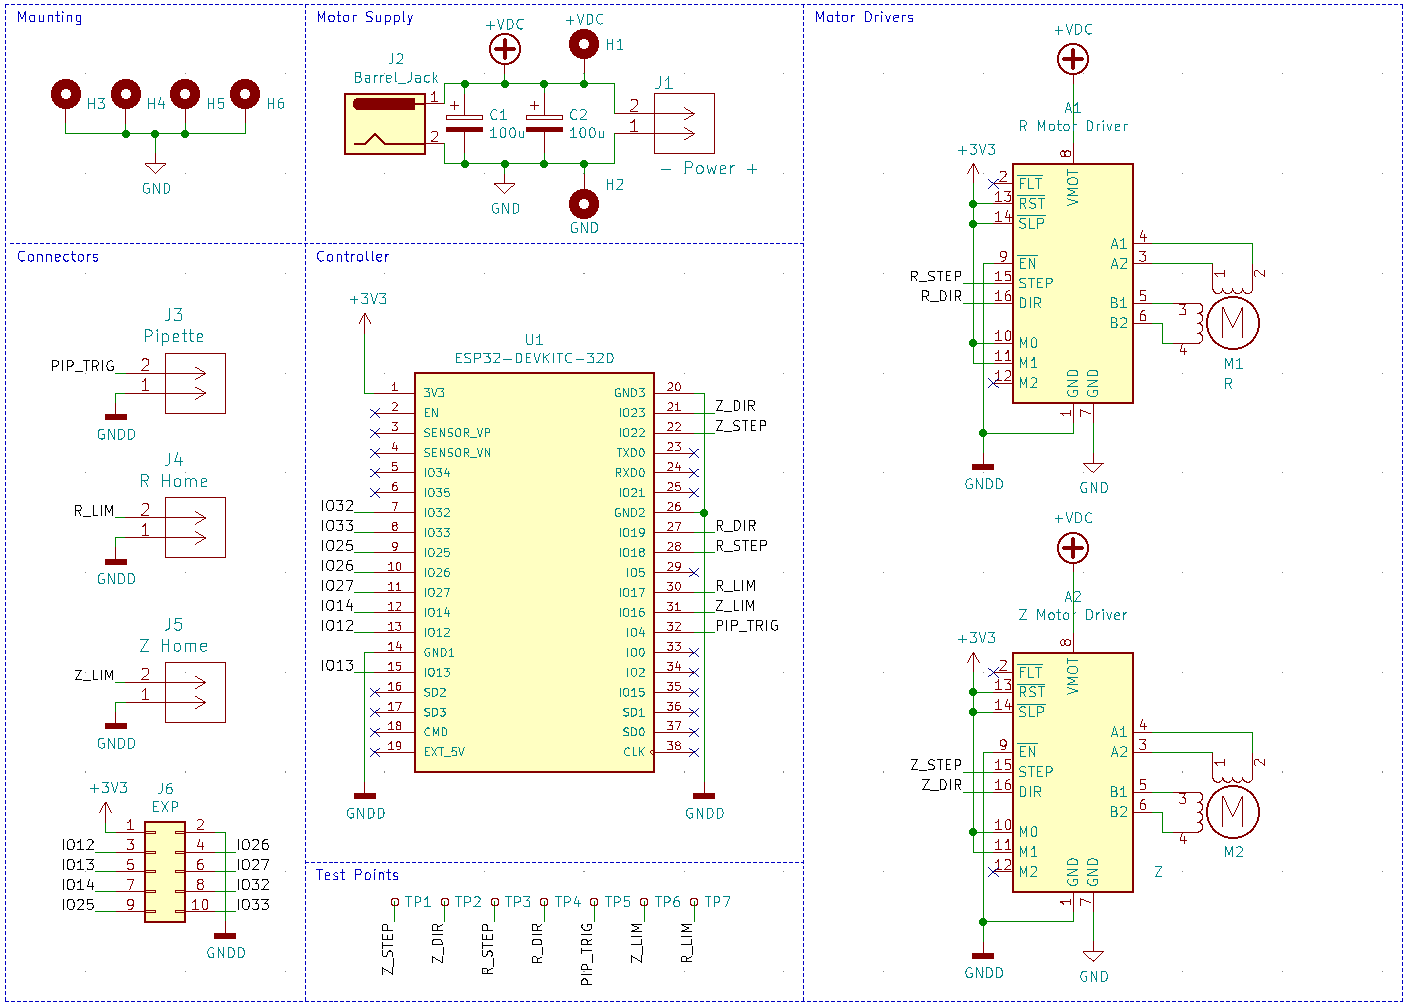
\includegraphics[height=0.3\textwidth]{img/schem.png}
    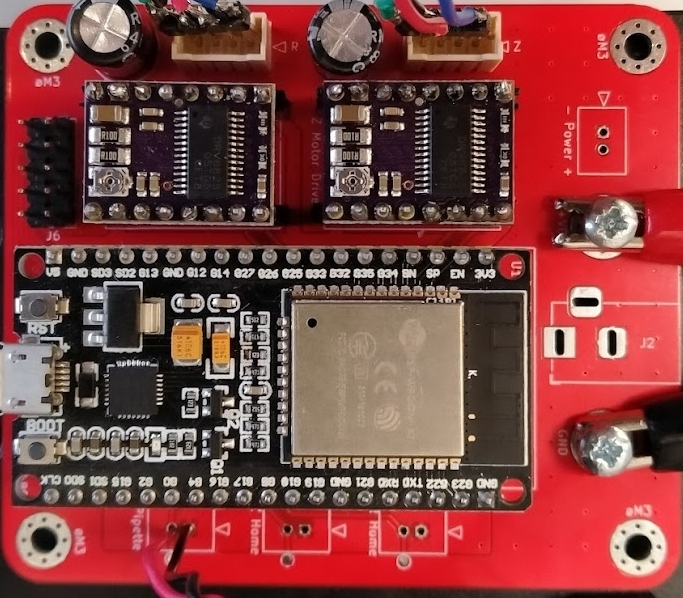
\includegraphics[height=0.3\textwidth]{img/control_pcb.png}
    \caption{Left: Controller Schematic and Right: Constructed PCB}
    \label{fig:schem_pcb}
\end{figure}

The figure\ref{fig:schem_pcb} shows the final electrical implementation and state the controller PCB (only partially populated due to COVID shipping delays). Note that this design included unfulfilled homing switch pads, as well as a 10 pin GPIO breakout for future expansion; i.e. external data acquisition syncing or other communication options.

The final consideration for this construction is whether the driver carriers require heatsinking or cooling. The DRV8825 driver IC has a maximum current rating of 2.5 A per coil, but the current sense resistors further limit the maximum current to 2.2 A, and the actual current you can deliver depends on how well you can keep the IC cool. The carrier’s printed circuit board is designed to draw heat out of the IC, but to supply more than approximately 1.5 A per coil, a heat sink or other cooling method is required. To obtain the systems requirements, both motors were supplied with a 15V DC motor voltage and the total current draw was tested at holding and under load.

This resulted in a max single driver holding current of 0.41A and a peak load current of 0.58A. 
This is well below the uncooled limit so no cooling solution was supplied.


\subsection{Motor Driving}
\subsection{Setup and Requirements}
To meet the driving requirements of the stepper motors outlined in this reports background [\ref{C:back}], preventing stalling and minimising harsh start stop behaviour that could cause unwanted vibrations, the controller and driver must be verified to be able to supply the step pulse train with ramping speeds and characterise the motors to ensure no steps are skipped. If this occurs the open loops control scheme will mean that the systems positional accuracy will fail.  

Test driving firmware was implemented on an ESP32 to validate its ability in producing the required pulse train step signal. The controller was required to produce N steps (pulses) at a set average speed, and ramp-up and down that pulse speed at the head and tail of that signal.

Set values of 200 steps forward and back, at a speed of 200 steps per second, with max acceleration of 800 steps per second per second:

These pulses were captured on a second microcontroller listening for falling edges to trigger an interrupt routine to record and display that data.

\subsection{Results}

\begin{figure}[h]
    \centering
    \begin{subfigure}{.45\textwidth}
        \centering
        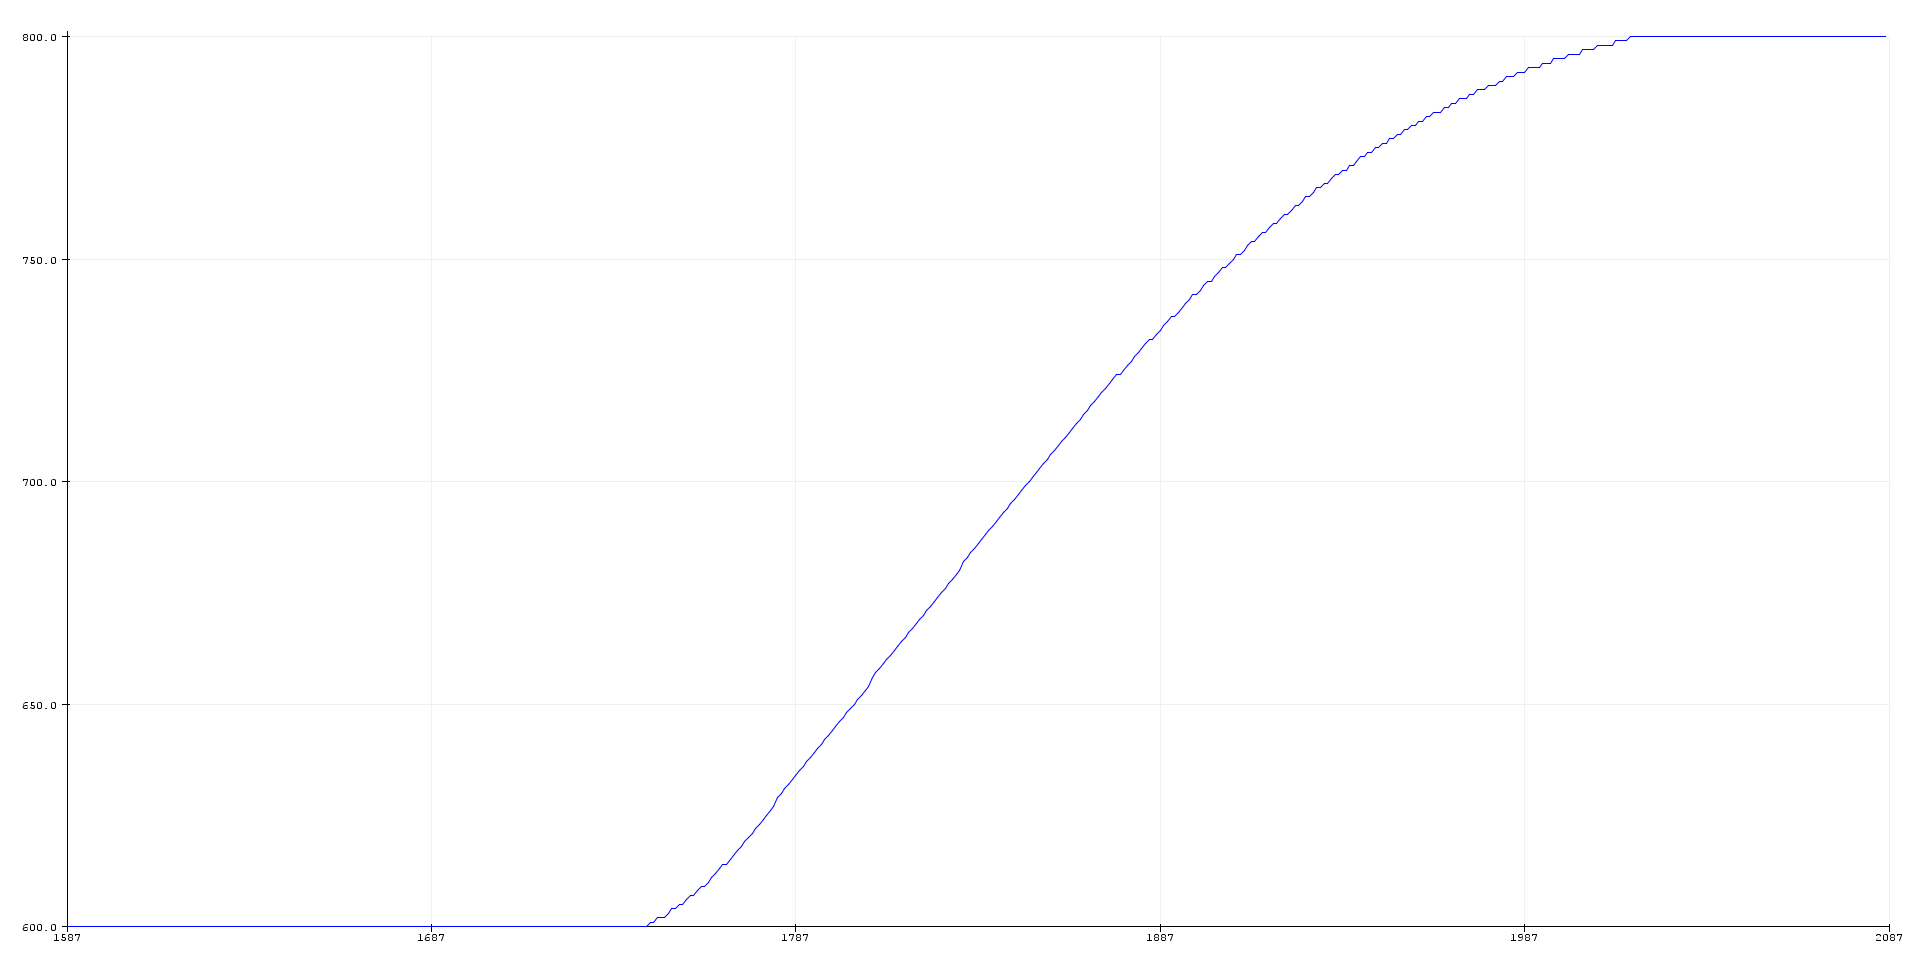
\includegraphics[width=0.8\linewidth]{img/stepper_pulses.PNG}
        \caption{Pulse Count}
    \end{subfigure}%
    \begin{subfigure}{.45\textwidth}
        \centering
        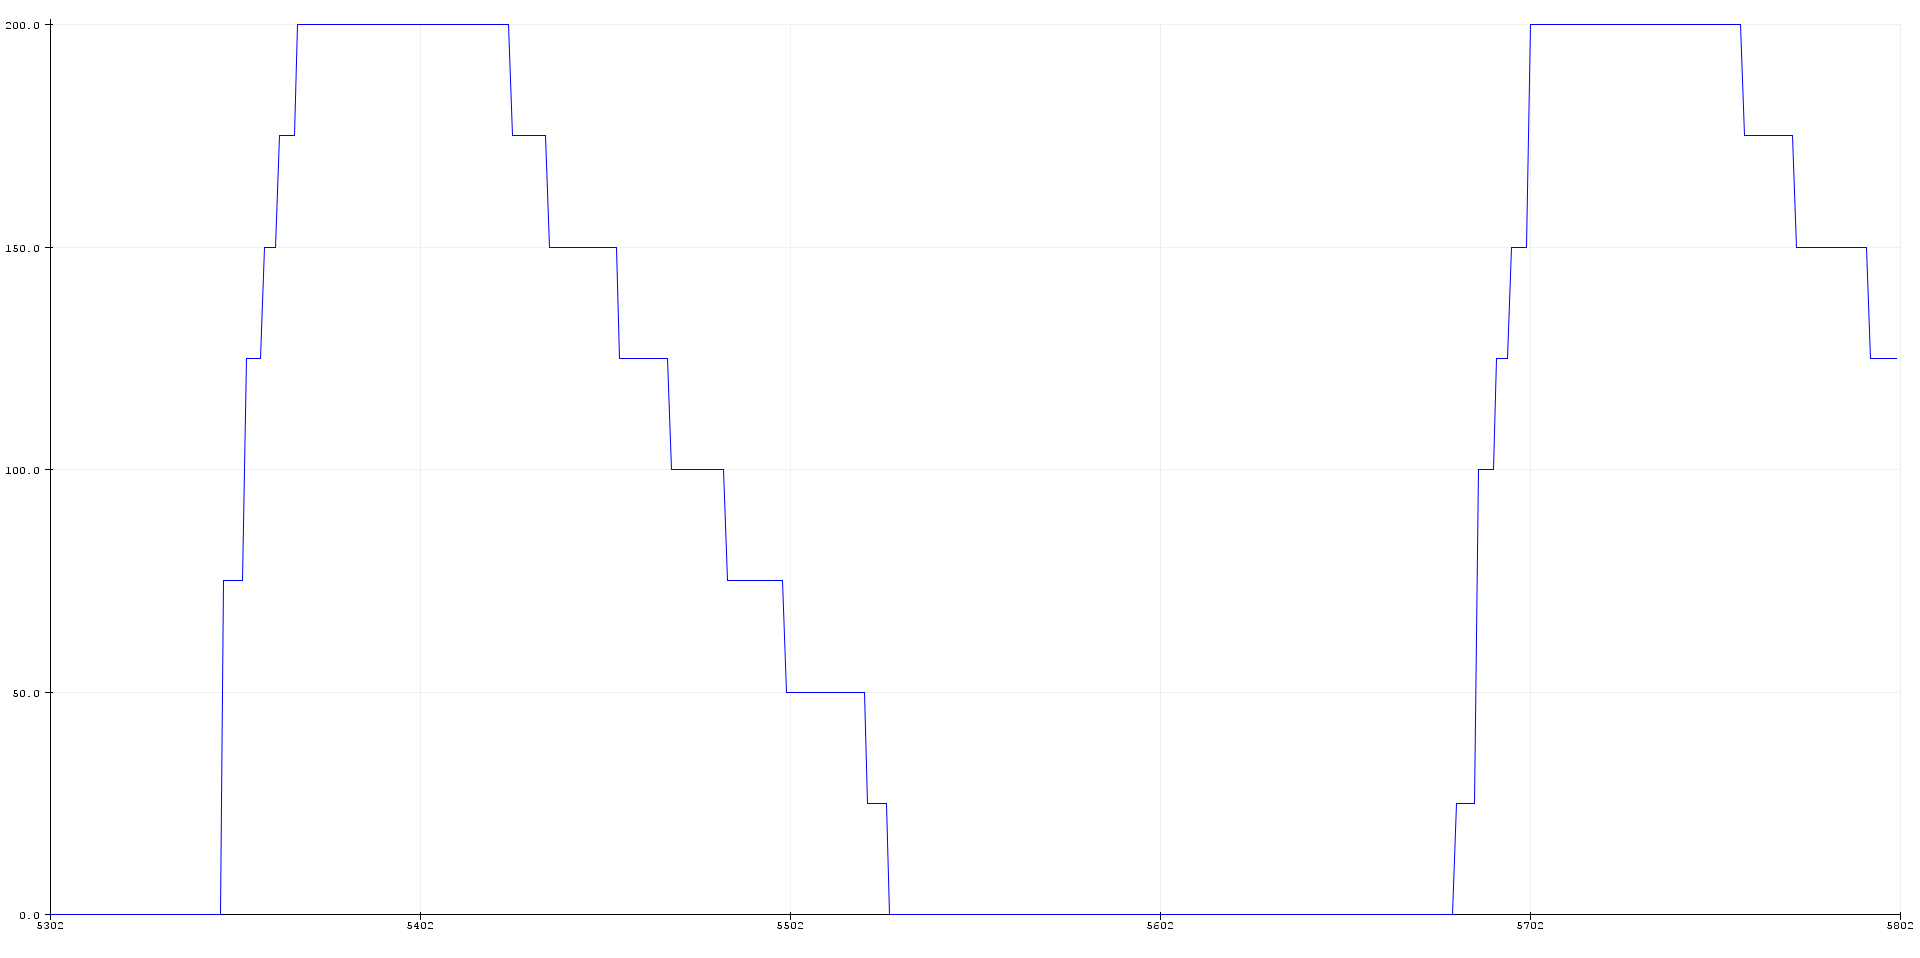
\includegraphics[width=0.8\linewidth]{img/stepper_pulse_acc.PNG}
        \caption{Pulses per Second}
    \end{subfigure}
    \caption{}
    \label{fig:code}
\end{figure}

Figure \ref{fig:code}:a shows a successfully produced signal of 200 pulses with an inferred acceleration at its head/tail. This speed ramping is better illustrated in figure \ref{fig:code}:b showing the stepping change in pulses per second over the course of the pulse train.

Additionally, it was found that these motors experiences some resonance and began skipping step when in 1:1 driving mode at the specific frequencies of 90Hz, 100Hz and 180Hz. This was solved by enabling the driver carrier's 1:32 microstepping mode and modifying the firmware to match.

\subsection{Pipette Triggering}

The pipette draws and dispenses liquid be using an internal DC motor to drive a leadscrew pressure chamber. This is controlled via a multi-function switch on the DC input daughter board. This daughterboard was required to be removed to gauge the signal requirement needed to trigger this event. 

\begin{figure}[h]
    \centering
    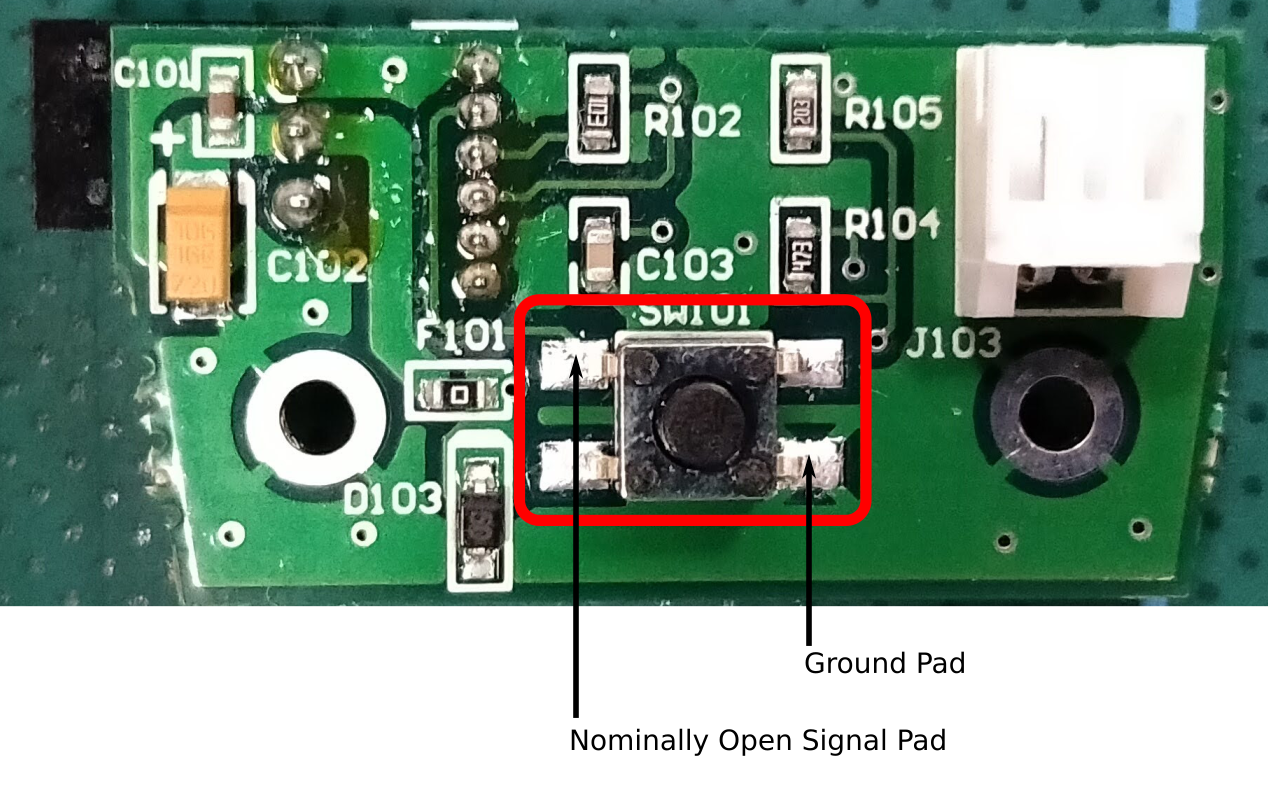
\includegraphics[width=0.4\textwidth]{img/trig_brd.png}
    \caption{E-Pipette dispensing trigger switch daughter board with exposed pads}
\end{figure}

From this investigation, it was determined the internal GPIO was connected to the nominally open (unconnected) pin of the switch. When actuated this line is pulled down to ground indicating a button press. This triggers 1 of 2 actions; Pipette wake-up or toggle leadscrew position, either dispensing or refilling the reservoir tip.   

To automate this process the nominally open pad was broken out to an output GPIO line on the controller and the ground was broken out and shared with the signal ground of the controller.

\section{Software}

\subsection{Instrumentation Controller}
ESP32 based system controller with serial interface for issuing commands. Provides functionality to:
\begin{itemize}
    \item Motorised stages, height and angular position
    \item e-Pipette droplet dispensing
\end{itemize}

The architectural approach for this controller is to provide an extendable and versatile command interface that allows for multiple input/control methods. For this reason, a continuous serial string input is polled for, parsed into internal library calls that control the motor driving signals and pipette actions. This allows the controller to be interfaced either directly with a text input serial command line, a LabView VISA serial control script or via a custom host side script.

\begin{figure*}[h]
    \centering
    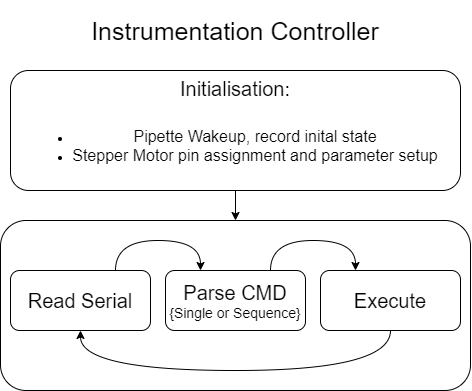
\includegraphics[width=0.4\textwidth]{img/software.png}
\end{figure*}

Upon boot, the firmware pings the pipette to wake it from sleep. Sets up symbolic motor objects to control signal generation with the correct micro steps, speed and acceleration terms. Then enters a command poll, parse and execute loop.

This command loop, translates real-world input units and translates them to the required step count.
For example to rotate the pipette by half a revolution the command \texttt{R 0.5} is sent, and to raise the pipette by 5mm, \texttt{Z 5mm}. The full command list is as follows: 

\begin{table}[]
    \begin{tabular}{|l|l|}
    \hline
    \texttt{ADJ R or Z {[}n\_steps{]}} & Debug command to allow individual stepping of motor \\ \hline
    \texttt{R {[}n\_revs{]} }       & Primary Pipette rotation, in revolutions            \\ \hline
    \texttt{Z {[}n\_mm{]}          }& Primary Z height adjustment, in mm                  \\ \hline
    \texttt{DEL {[}delay\_time{]}  }& Add time delay in ms                                \\ \hline
    \texttt{PIP {[}UP|DOWN{]}      }& Draw liquid (UP) or dispense (DOWN)                 \\ \hline
    \end{tabular}
    \end{table}
    
Internally the firmware keeps track of the last pipette action to ensure the user does not accidentally dispense or draw liquid.

To enable setup and tuning as well as full experiment automation there are two command input modes. Individual and Sequence. To enter a sequence, the special command \texttt{SEQ} is sent follows be semicolon-separated commands, \texttt{Z -5; PIP UP; Z 5; R 0.25; DEL 200; PIP DOWN; Z -4; Z 4; R -0.25; END;}.

This firmware produces two main parameters that are available for tuning when evaluating the performance of the integrated system: The step signals pulse speed, and its ramping acceleration.

\section{Environmental Monitoring}

\begin{figure}[h]
    \centering
    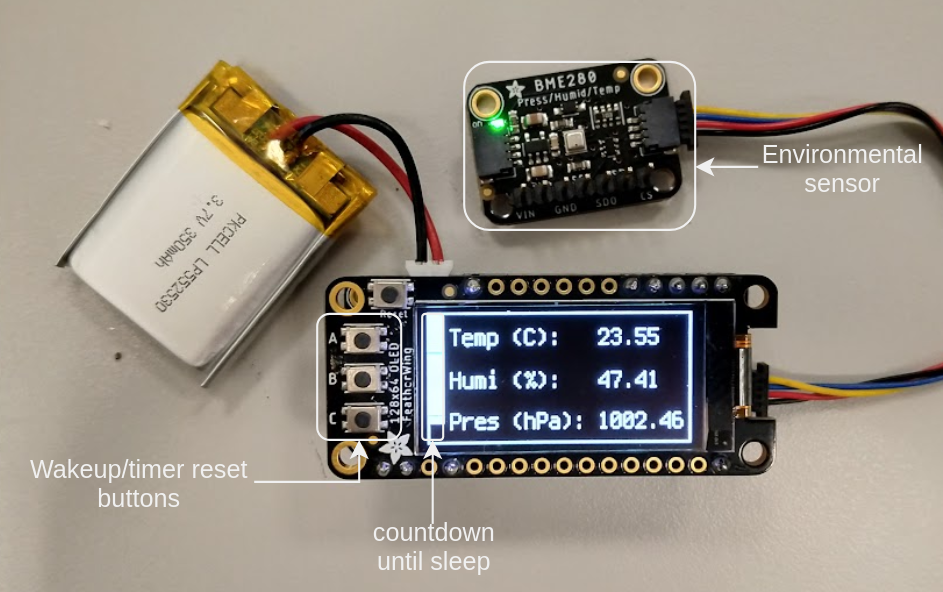
\includegraphics[width=0.4\textwidth]{img/env_mon.png}
    \caption{Implemented Environmental Monitor}
\end{figure}

The design values speed and quick integration, so assembly was plugin-play. The primary work down was the power management and data-collection software. The BME280 and OLED screen are attached to the I2C bus with unique addresses. These are polled to retrieve prefiltered temperature, pressure and humidity data and pushed to the screen.

\subsection*{Low Power}
As the system is portable and powered only by a single cell LiPO battery, long life is more of a requirement than continuous display, as the data is only needed to be noted at the beginning of an experiment. To achieve the firmware attaches button alarm interrupts to OLED screens buttons and counts downs an internal timer. Upon timeout this firmware clears the OLED, places the screen and BME in sleep mode. These will now draw $5\mu A$ and $2 \mu A$ respectively. The RP2040 itself then enters deep sleep, clearing memory and shutting down most of its hardware, achieving $180\mu A$ of draw. 

\section{Full System}

\begin{figure}[h]
    \centering
    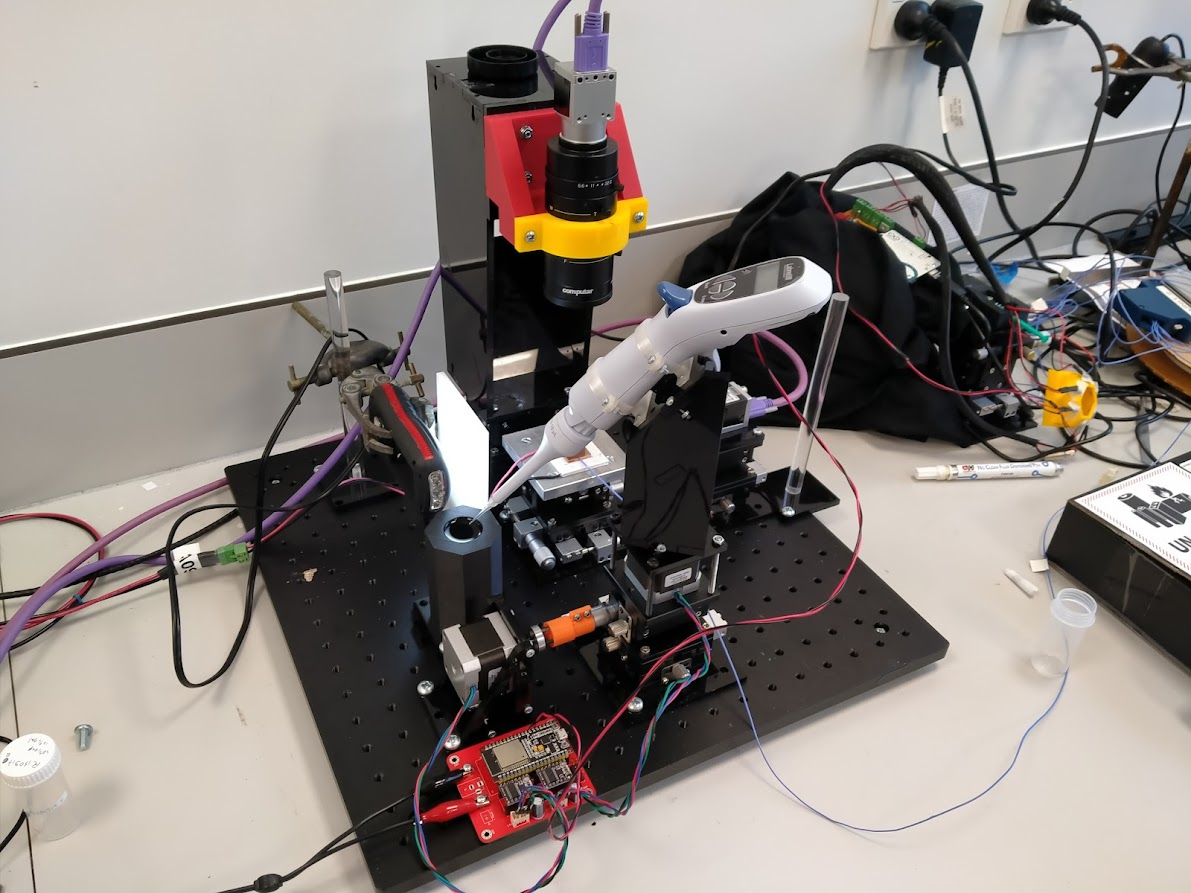
\includegraphics[height=0.3\textwidth]{img/full_sys.jpg}
    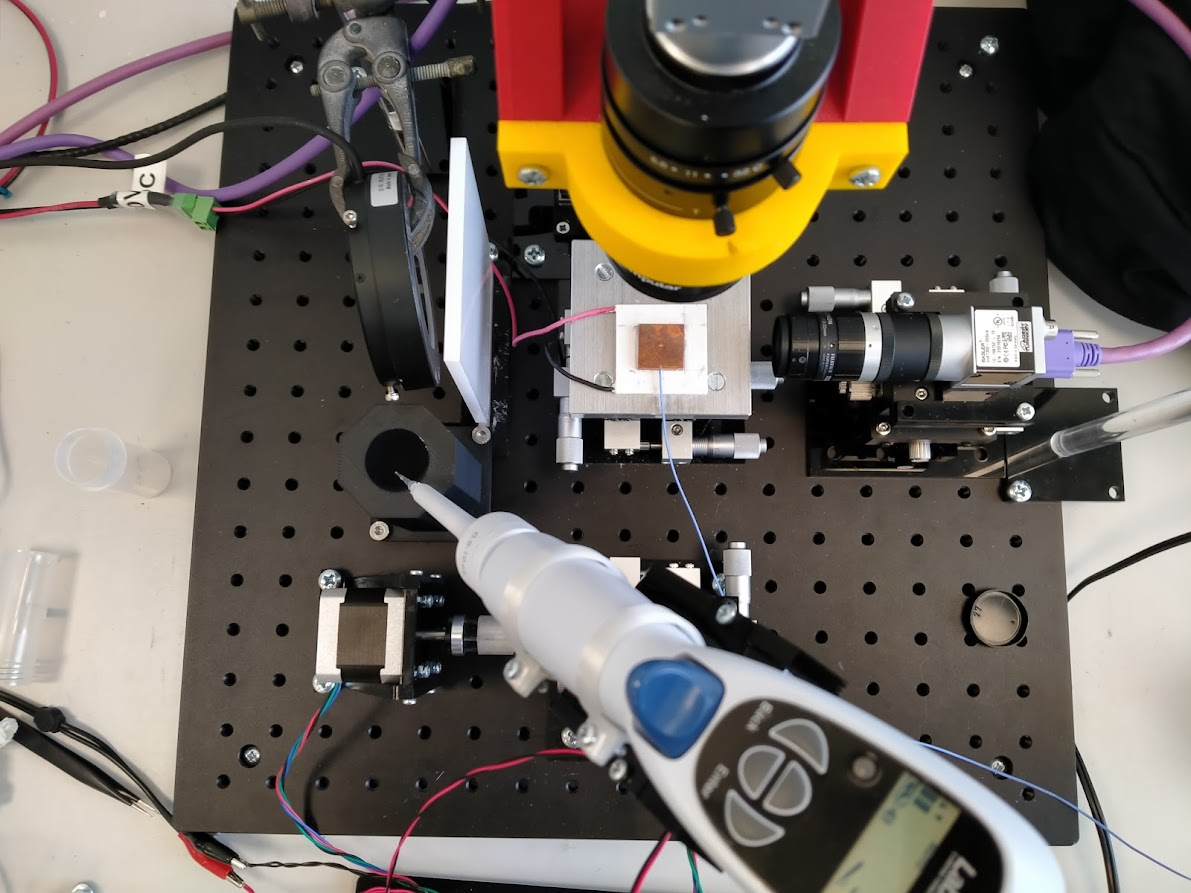
\includegraphics[height=0.3\textwidth]{img/impl_sys_top.jpg}
    \caption{Full System}
\end{figure}

Fully integrated, this system is assembled on an optical breadboard with an assortment of adjustable XYZ micrometer stages; camera mounts, backlight and diffusers, a liquid reservoir and a central substrate stack. The procedure this instrumentation follows is: lower pipette tip into the static reservoir and draw pre-programmed volume into tip, raise pipette to the required height, rotate to depositing point, dispense droplet and pause, lower and raise pipette to deposit drop on substrate, rotate pipette clear of camera view.